%% LyX 2.4.4 created this file.  For more info, see https://www.lyx.org/.
%% Do not edit unless you really know what you are doing.
\documentclass[english]{article}
\usepackage[T1]{fontenc}
\usepackage[latin9]{inputenc}
\usepackage{cancel}

\makeatletter
%%%%%%%%%%%%%%%%%%%%%%%%%%%%%% User specified LaTeX commands.
\usepackage{multicol}

\usepackage{tikz}
\usetikzlibrary{calc}
\usetikzlibrary{plotmarks}
\usepackage{pgfplots}
\pgfplotsset{compat=newest}

\usepackage{calc}
\usepackage[nomessages]{fp}

\usepackage{advdate}    % Advancing/saving dates
\usepackage{datetime}   % Dates formatting
\usepackage{datenumber} % Counters for dates
\usepackage[super]{nth}

\usepackage{etex}

\makeatother

\usepackage{babel}
\begin{document}
%%%%A or B%%%%%
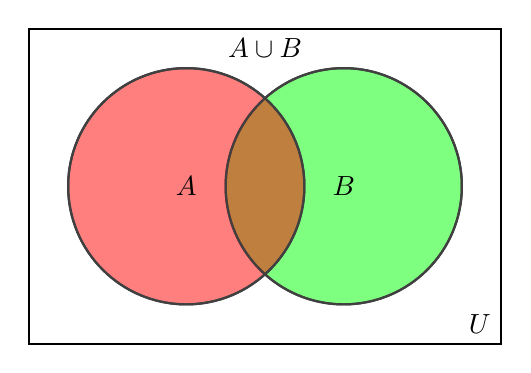
\begin{tikzpicture} 
	\def\circleA{(0,0) circle (1.5)} %A
	\def\circleB{(0:2) circle (1.5)} %B

	\colorlet{circle edgeA}{black!75} 
	\colorlet{circle areaA}{red!100}
	\colorlet{circle edgeB}{black!75} 
	\colorlet{circle areaB}{green!100}

	\tikzset{
		filledA/.style={fill=circle areaA, draw=circle edgeA, thick},
		filledB/.style={fill=circle areaB, draw=circle edgeB, thick},
		outlineA/.style={draw=circle edgeA, thick},
		outlineB/.style={draw=circle edgeB, thick},
	}
	
	\begin{scope}[fill opacity=0.5]         
			\fill[filledB] \circleB;    
			\fill[filledA] \circleA;
	\end{scope}

	\draw[outlineA] \circleA node {$A$}; 
	\draw[outlineB] \circleB node {$B$}; 
	\node[anchor=south] at (current bounding box.north) {$A \cup B$}; 
	\draw[thick] (-2,-2) rectangle (4,2) node[anchor=south east] at (current bounding box.south east) {$U$}; 
\end{tikzpicture} 

%%%%A and B%%%%%
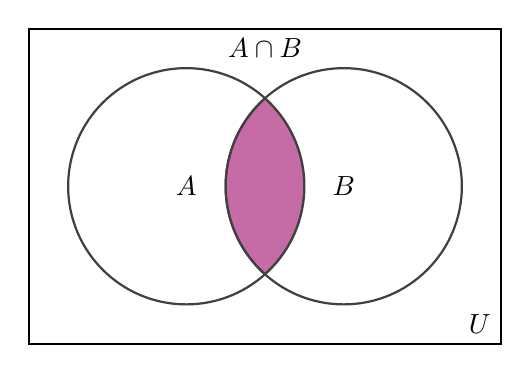
\begin{tikzpicture} 
	\def\circleA{(0,0) circle (1.5)} %A
	\def\circleB{(0:2) circle (1.5)} %B

	\colorlet{circle edgeA}{black!75} 
	\colorlet{circle areaA}{red!100}
	\colorlet{circle edgeB}{black!75} 
	\colorlet{circle areaB}{blue!100}

	\tikzset{
		filledA/.style={fill=circle areaA, draw=circle edgeA, thick},
		filledB/.style={fill=circle areaB, draw=circle edgeB, thick},
		outlineA/.style={draw=circle edgeA, thick},
		outlineB/.style={draw=circle edgeB, thick},
	}
	
	\begin{scope}[fill opacity=0.35]    
		\clip \circleA;     
			\fill[filledB] \circleB;
		\clip \circleB;     
			\fill[filledA] \circleA;
	\end{scope}

	\draw[outlineA] \circleA node {$A$}; 
	\draw[outlineB] \circleB node {$B$}; 
	\node[anchor=south] at (current bounding box.north) {$A \cap B$}; 
	\draw[thick] (-2,-2) rectangle (4,2) node[anchor=south east] at (current bounding box.south east) {$U$}; 
\end{tikzpicture} 

%%%%A compliment%%%%%
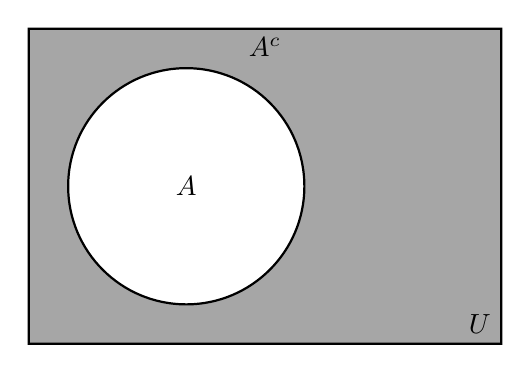
\begin{tikzpicture} 
	\def\circleA{(0,0) circle (1.5)} %A
	\def\circleB{(0:2) circle (1.5)} %B

	\colorlet{circle edgeA}{black!75} 
	\colorlet{circle areaA}{red!100}
	\colorlet{circle edgeB}{black!75} 
	\colorlet{circle areaB}{blue!100}

	\tikzset{
		filledA/.style={fill=circle areaA, draw=circle edgeA, thick},
		filledB/.style={fill=circle areaB, draw=circle edgeB, thick},
		outlineA/.style={draw=circle edgeA, thick},
		outlineB/.style={draw=circle edgeB, thick},
	}

	\draw[thick,fill=black!35,even odd rule] %%even odd rule draws compliment of next draw commands%%
		(-2,-2) rectangle (4,2) node[anchor=south east] at (current bounding box.south east) {$U$} 
		\circleA node {$A$};
	\node[below] at (current bounding box.north) {$A^{c}$}; 

\end{tikzpicture} 

\newcommand{\vennScale}{0.5}

%%%%A U B%%%%%
\begin{tikzpicture}[scale=\vennScale]
	\def\circleA{(0,0) circle (1.5)} %A
	\def\circleB{(0:2) circle (1.5)} %B

	\colorlet{circle edgeA}{black!75} 
	\colorlet{circle areaA}{red!50}
	\colorlet{circle edgeB}{black!75} 
	\colorlet{circle areaB}{red!50}

	\tikzset{
		filledA/.style={fill=circle areaA, draw=circle edgeA, thick},
		filledB/.style={fill=circle areaB, draw=circle edgeB, thick},
		outlineA/.style={draw=circle edgeA, thick},
		outlineB/.style={draw=circle edgeB, thick},
	}
	
	\begin{scope}[fill opacity=1.0]         
			\fill[filledB] \circleB;    
			\fill[filledA] \circleA;
	\end{scope}

	\draw[outlineA] \circleA node {$A$}; 
	\draw[outlineB] \circleB node {$B$}; 
	%\node[anchor=south] at (current bounding box.north) {$A \cap B$}; 
	\draw[thick] (-2,-2) rectangle (4,2) node[anchor=south east] at (current bounding box.south east) {$U$}; 
\end{tikzpicture} 

%%%%A n B%%%%%
\begin{tikzpicture}[scale=\vennScale]
	\def\circleA{(0,0) circle (1.5)} %A
	\def\circleB{(0:2) circle (1.5)} %B

	\colorlet{circle edgeA}{black!75} 
	\colorlet{circle areaA}{red!50}
	\colorlet{circle edgeB}{black!75} 
	\colorlet{circle areaB}{red!50}

	\tikzset{
		filledA/.style={fill=circle areaA, draw=circle edgeA, thick},
		filledB/.style={fill=circle areaB, draw=circle edgeB, thick},
		outlineA/.style={draw=circle edgeA, thick},
		outlineB/.style={draw=circle edgeB, thick},
	}
	
	\begin{scope}[fill opacity=1.0]    
		\clip \circleA;     
			\fill[filledB] \circleB;
		\clip \circleB;     
			\fill[filledA] \circleA;
	\end{scope}

	\draw[outlineA] \circleA node {$A$}; 
	\draw[outlineB] \circleB node {$B$}; 
	%\node[anchor=south] at (current bounding box.north) {$A \cap B$}; 
	\draw[thick] (-2,-2) rectangle (4,2) node[anchor=south east] at (current bounding box.south east) {$U$}; 
\end{tikzpicture} 

%%%%A'%%%%%
\begin{tikzpicture}[scale=\vennScale]
	\def\circleA{(0,0) circle (1.5)} %A
	\def\circleB{(0:2) circle (1.5)} %B

	\colorlet{circle edgeA}{black!75} 
	\colorlet{circle areaA}{red!100}
	\colorlet{circle edgeB}{black!75} 
	\colorlet{circle areaB}{blue!100}

	\tikzset{
		filledA/.style={fill=circle areaA, draw=circle edgeA, thick},
		filledB/.style={fill=circle areaB, draw=circle edgeB, thick},
		outlineA/.style={draw=circle edgeA, thick},
		outlineB/.style={draw=circle edgeB, thick},
	}

	\draw[thick,fill=red!50,even odd rule] %%even odd rule draws complement of next draw commands%%
		(-2,-2) rectangle (4,2) node[anchor=south east] at (current bounding box.south east) {$U$} 
		\circleA node {$A$};
	\draw[outlineB] \circleB node {$B$}; 
	%\node[below=1pt] at (current bounding box.north) {\footnotesize $A'$}; 

\end{tikzpicture} 

%%%%B'%%%%%
\begin{tikzpicture}[scale=\vennScale]
	\def\circleA{(0,0) circle (1.5)} %A
	\def\circleB{(0:2) circle (1.5)} %B

	\colorlet{circle edgeA}{black!75} 
	\colorlet{circle areaA}{red!100}
	\colorlet{circle edgeB}{black!75} 
	\colorlet{circle areaB}{blue!100}

	\tikzset{
		filledA/.style={fill=circle areaA, draw=circle edgeA, thick},
		filledB/.style={fill=circle areaB, draw=circle edgeB, thick},
		outlineA/.style={draw=circle edgeA, thick},
		outlineB/.style={draw=circle edgeB, thick},
	}

	\draw[thick,fill=red!50,even odd rule] %%even odd rule draws complement of next draw commands%%
		(-2,-2) rectangle (4,2) node[anchor=south east] at (current bounding box.south east) {$U$} 
		\circleB node {$B$};
	\draw[outlineA] \circleA node {$A$}; 
	%\node[below=1pt] at (current bounding box.north) {\footnotesize $A'$}; 

\end{tikzpicture} 

%%%%A n B'%%%%%
\begin{tikzpicture}[scale=\vennScale]
	\def\circleA{(0,0) circle (1.5)} %A
	\def\circleB{(0:2) circle (1.5)} %B

	\colorlet{circle edgeA}{black!75} 
	\colorlet{circle areaA}{red!50}
	\colorlet{circle edgeB}{black!75} 
	\colorlet{circle areaB}{red!50}

	\tikzset{
		filledA/.style={fill=circle areaA, draw=circle edgeA, thick},
		filledB/.style={fill=circle areaB, draw=circle edgeB, thick},
		outlineA/.style={draw=circle edgeA, thick},
		outlineB/.style={draw=circle edgeB, thick},
	}
	
	\begin{scope}[fill opacity=1.0]    
		\fill[circle areaA] \circleA;
		\clip \circleA;     
			\fill[white] \circleB;
		%\clip \circleB;     
			%\fill[filledA] \circleA;
	\end{scope}

	\draw[outlineA] \circleA node {$A$}; 
	\draw[outlineB] \circleB node {$B$}; 
	%\node[anchor=south] at (current bounding box.north) {$A \cap B$}; 
	\draw[thick] (-2,-2) rectangle (4,2) node[anchor=south east] at (current bounding box.south east) {$U$}; 
\end{tikzpicture} 

%%%%A'U B%%%%%
\begin{tikzpicture}[scale=\vennScale]
	\def\circleA{(0,0) circle (1.5)} %A
	\def\circleB{(0:2) circle (1.5)} %B

	\colorlet{circle edgeA}{black!75} 
	\colorlet{circle areaA}{red!100}
	\colorlet{circle edgeB}{black!75} 
	\colorlet{circle areaB}{blue!100}

	\tikzset{
		filledA/.style={fill=circle areaA, draw=circle edgeA, thick},
		filledB/.style={fill=circle areaB, draw=circle edgeB, thick},
		outlineA/.style={draw=circle edgeA, thick},
		outlineB/.style={draw=circle edgeB, thick},
	}

	\draw[fill=red!50]\circleB node {$B$};

	\draw[thick,fill=red!50,even odd rule] %%even odd rule draws complement of next draw commands%%
		(-2,-2) rectangle (4,2) node[anchor=south east] at (current bounding box.south east) {$U$}
		\circleA node {$A$};
	%\node[below=1pt] at (current bounding box.north) {\footnotesize $A'$};
	
	\draw[outlineB] \circleB node {$B$}; 

\end{tikzpicture} 

%%%%(A n B)'%%%%%
\begin{tikzpicture}[scale=\vennScale]
	\def\circleA{(0,0) circle (1.5)} %A
	\def\circleB{(0:2) circle (1.5)} %B

	\colorlet{circle edgeA}{black!75} 
	\colorlet{circle areaA}{white}
	\colorlet{circle edgeB}{black!75} 
	\colorlet{circle areaB}{white}

	\tikzset{
		filledA/.style={fill=circle areaA, draw=circle edgeA, thick},
		filledB/.style={fill=circle areaB, draw=circle edgeB, thick},
		outlineA/.style={draw=circle edgeA, thick},
		outlineB/.style={draw=circle edgeB, thick},
	}
	\draw[fill=red!50] (-2,-2) rectangle (4,2);

	\begin{scope}[fill opacity=1.0]    
		\clip \circleA;     
			\fill[filledB] \circleB;
		\clip \circleB;     
			\fill[filledA] \circleA;
	\end{scope}

	\draw[outlineA] \circleA node {$A$}; 
	\draw[outlineB] \circleB node {$B$}; 
	%\node[anchor=south] at (current bounding box.north) {$A \cap B$}; 
	\draw[thick] (-2,-2) rectangle (4,2) node[anchor=south east] at (current bounding box.south east) {$U$}; 
\end{tikzpicture} 

%%%%(AUB)' complement%%%%%
\begin{tikzpicture}[scale=\vennScale]
	\def\circleA{(0,0) circle (1.5)} %A
	\def\circleB{(0:2) circle (1.5)} %B

	\colorlet{circle edgeA}{black!75} 
	\colorlet{circle areaA}{red!100}
	\colorlet{circle edgeB}{black!75} 
	\colorlet{circle areaB}{blue!100}

	\tikzset{
		filledA/.style={fill=circle areaA, draw=circle edgeA, thick},
		filledB/.style={fill=circle areaB, draw=circle edgeB, thick},
		outlineA/.style={draw=circle edgeA, thick},
		outlineB/.style={draw=circle edgeB, thick},
	}

		\draw[thick,fill=red!50,even odd rule] %%even odd rule draws complement of next draw commands%%
			(-2,-2) rectangle (4,2) node[anchor=south east] at (current bounding box.south east) {$U$}
			\circleA node {$A$} \circleB node {$B$};

		\scope 
			\clip (0,0) circle (1.5);%%why can't i use circleA?
			\fill[white] (0:2) circle (1.5); 
		\endscope
		
	%\node[below=1pt] at (current bounding box.north) {\footnotesize $(A \cup B$)'}; 

\end{tikzpicture} 

%%%3 empty circles with labels%%%%
\def\firstcircle{(90:1.75cm) circle (2.5cm)} 
\def\secondcircle{(210:1.75cm) circle (2.5cm)} 
\def\thirdcircle{(330:1.75cm) circle (2.5cm)}

\begin{tikzpicture}[scale=.9]    
\begin{scope}     
	\fill[white]\firstcircle;       
	\fill[white] \secondcircle;       
	\fill[white] \thirdcircle;     
\end{scope}     
\begin{scope}
	\clip 
	\secondcircle;       
	\fill[white] 
	\firstcircle;     
\end{scope}     
\begin{scope}       
	\clip 
	\secondcircle;       
	\fill[white] 
	\thirdcircle;     
\end{scope}     
\begin{scope}       
	\clip 
	\firstcircle;       
	\fill[white] 
	\thirdcircle;     
\end{scope}     
\begin{scope}       
	\clip \firstcircle;       
	\clip \secondcircle;       
	\fill[white] \thirdcircle;     
\end{scope}     
\draw 
	\firstcircle node[text=black] {$D$} node[above=10pt] {$10$};     
\draw 
	\secondcircle node [text=black,below left] {$C$} node[below left=10pt] {$10$};     
\draw 
	\thirdcircle node [text=black,below right] {$F$} node[below right=10pt] {$10$};     
\begin{scope}[font=\small]       
	\node(0,0) {$25$}; %AnBnC       
	\draw(30:1.5cm) node {$15$}; %AnC       
	\draw(150:1.5cm) node {$20$}; %AnB       
\draw(270:1.5cm) node {$5$}; %BnC    
\end{scope}

\draw[thick] (-4.8,-3.55) rectangle (4.75,4.4) node[anchor=south east] at (current bounding box.south east) {$U$} node[anchor=north west] at (current bounding box.north west) {$105$}; 

\end{tikzpicture}

%%%%3 colored circles with labels%%%
\def\firstcircle{(90:1.75cm) circle (2.5cm)} 
\def\secondcircle{(210:1.75cm) circle (2.5cm)} 
\def\thirdcircle{(330:1.75cm) circle (2.5cm)}

\begin{tikzpicture}[scale=.9]    
\begin{scope}     
	\fill[red!50]\firstcircle; %A    
	\fill[blue!50] \secondcircle; %B       
	\fill[yellow!50] \thirdcircle; %C    
\end{scope}     
\begin{scope} %%AnB only
	\clip 
	\secondcircle;       
	\fill[purple!50] 
	\firstcircle;     
\end{scope}     
\begin{scope} %%BnC only    
	\clip 
	\secondcircle;       
	\fill[green!50] 
	\thirdcircle;     
\end{scope}     
\begin{scope} %%AnC only    
	\clip 
	\firstcircle;       
	\fill[orange!50] 
	\thirdcircle;     
\end{scope}     
\begin{scope} %%AnBnC     
	\clip \firstcircle;       
	\clip \secondcircle;       
	\fill[blue!50!red!50!yellow!50] \thirdcircle;     
\end{scope}     
\draw 
	\firstcircle node[text=black] {$A$} node[above=10pt] {$$};     
\draw 
	\secondcircle node [text=black,below left] {$B$} node[below left=10pt] {$$};     
\draw 
	\thirdcircle node [text=black,below right] {$C$} node[below right=10pt] {$$};     
\begin{scope}[font=\small]       
	\node(0,0) {\footnotesize $A\cap B\cap C$}; %AnBnC       
	\draw(30:1.5cm) node {$A\cap C$}; %AnC       
	\draw(150:1.5cm) node {$A\cap B$}; %AnB       
\draw(270:1.5cm) node {$B\cap C$}; %BnC    
\end{scope}

\draw[thick] (-4.8,-3.55) rectangle (4.75,4.4) node[anchor=south east] at (current bounding box.south east) {$U$} node[anchor=north west] at (current bounding box.north west) {$105$}; 

\end{tikzpicture}

%%some commands for the graphs%%%
\newcommand{\xmax}{0}
\newcommand{\xmin}{-\xmax}
\newcommand{\xstep}{0}
\newcommand{\ymax}{0}
\newcommand{\ymin}{-\ymax}
\newcommand{\ystep}{0} 
\newcommand{\Fx}{x}
\newcommand{\Gx}{x}
\newcommand{\samples}{500}

%%%%%%piecewise function%%%%
\renewcommand{\Fx}{x+4}
\renewcommand{\Gx}{-2*x+4}
\renewcommand{\xmax}{7}
\renewcommand{\xmin}{-7}
\renewcommand{\xstep}{0} %must be xmin+n
\renewcommand{\ymax}{5}
\renewcommand{\ymin}{-5}
\renewcommand{\ystep}{-} %must be ymin+n
%%%%%%%
\begin{tikzpicture}
\begin{axis}[%height=5cm, 
	width=6cm,
	axis equal,
	axis lines=middle,
	%axis line style={-latex}, 
	xmin=\xmin,xmax=\xmax, 
	ymin=\ymin,ymax=\ymax,
	%restrict y to domain=-1:10,
	%no markers, 
	%ticks=none,
	%minor grid style={gray!25},
	%major grid style={black!50},
	minor x tick num={4},
	minor y tick num={4},
	grid=both,
	xlabel={$x$},ylabel={$y$}, 
	%every axis x label/.append style={anchor=north}, 
	%every axis y label/.append style={anchor=east}, 
	]

	%\addplot+[domain=1:3,fill,black!30!white]{\Fx} \closedcycle;
	%\addplot+[domain=1:3,fill,black!30!white]{\Fx} \closedcycle;

	%\draw[thick,black,dashed] (axis cs:1,0) node[below] {$1$} -- (axis cs:1,1) ;
	%\draw[thick,black,dashed] (axis cs:3,0) node[below] {$3$} -- (axis cs:3,1.73205);
	
	\addplot[domain=-4:0,thick,smooth,red,samples=\samples]{\Fx} node[above,pos=.35,yshift=10pt] {$f(x)$};
	\addplot[domain=0:4,thick,smooth,red,samples=\samples]{\Gx} node[above,pos=.35,yshift=5pt] {$$}; 
	
	\node at (axis cs:2,.75) {$R$};
\end{axis}
\end{tikzpicture}

%%%%%%%%area under curve%%%%
\renewcommand{\Fx}{x^(1/2)}
\renewcommand{\xmax}{5}
\renewcommand{\xmin}{-1}
\renewcommand{\xstep}{0} %must be xmin+n
\renewcommand{\ymax}{2}
\renewcommand{\ymin}{-.35}
\renewcommand{\ystep}{-} %must be ymin+n
%%%%%%%
\begin{tikzpicture}
\begin{axis}[height=4cm, 
	width=5cm, 
	axis lines=middle,
	%axis line style={-latex}, 
	xmin=\xmin,xmax=\xmax, 
	ymin=\ymin,ymax=\ymax,
	%restrict y to domain=-1:10,
	no markers, 
	ticks=none,
	xlabel={$x$},ylabel={$y$}, 
	%every axis x label/.append style={anchor=north}, 
	%every axis y label/.append style={anchor=east}, 
	area style,tension=0.08]

	\addplot+[domain=1:3,fill,black!30!white]{\Fx} \closedcycle;
	\addplot+[domain=1:3,fill,black!30!white]{\Fx} \closedcycle;

	\draw[thick,black,dashed] (axis cs:1,0) node[below] {$1$} -- (axis cs:1,1) ;
	\draw[thick,black,dashed] (axis cs:3,0) node[below] {$3$} -- (axis cs:3,1.73205);
	
	\addplot[domain=0:\xmax,thick,smooth,red,samples=\samples]{\Fx} node[above,pos=.35,yshift=3pt] {$f(x)$}; 
	
	\node at (axis cs:2,.75) {$R$};
\end{axis}
\end{tikzpicture}

%%%%area between curves%%%
\renewcommand{\xmax}{15}
\renewcommand{\xmin}{-4}
\renewcommand{\xstep}{0} %must be xmin+n
\renewcommand{\ymax}{15}
\renewcommand{\ymin}{-3}
\renewcommand{\ystep}{-} %must be ymin+n
%%%%%%%
\begin{tikzpicture}
\begin{axis}[height=4cm, 
	width=5cm, 
	axis lines=middle,
	%axis line style={-latex}, 
	xmin=\xmin,xmax=\xmax, 
	ymin=\ymin,ymax=\ymax,
	%restrict y to domain=-1:10,
	no markers, 
	ticks=none,
	xlabel={$x$},ylabel={$y$}, 
	%every axis x label/.append style={anchor=north}, 
	%every axis y label/.append style={anchor=east}, 
	area style,tension=0.08]

\addplot+[domain=3:12,fill,black!30!white]{1*cos(deg(x/2))+10} \closedcycle;
	%\addplot+[domain=3:12,fill,black!30!white]{1*cos(deg(x/2.7))+3} \closedcycle;

	\draw[thick,black,dashed] (axis cs:3,0) node[below] {$a$} -- (axis cs:3,10.0707) ;
	\draw[thick,black,dashed] (axis cs:12,0) node[below] {$b$} -- (axis cs:12,10.9602);
	
	\addplot[domain=\xmin+1:\xmax,thick,smooth,red,samples=\samples]{1*cos(deg(x/2))+10} node[above,pos=.04] {$f(x)$}; 
	\addplot[domain=\xmin+1:\xmax,thick,smooth,blue,samples=\samples]{1*cos(deg(x/2.7))+3} node[above,pos=.04] {$g(x)$};

	\node at (axis cs:7.5,6) {$R$};
\end{axis}
\end{tikzpicture}
\end{document}
